\documentclass[1p]{elsarticle_modified}
%\bibliographystyle{elsarticle-num}

%\usepackage[colorlinks]{hyperref}
%\usepackage{abbrmath_seonhwa} %\Abb, \Ascr, \Acal ,\Abf, \Afrak
\usepackage{amsfonts}
\usepackage{amssymb}
\usepackage{amsmath}
\usepackage{amsthm}
\usepackage{scalefnt}
\usepackage{amsbsy}
\usepackage{kotex}
\usepackage{caption}
\usepackage{subfig}
\usepackage{color}
\usepackage{graphicx}
\usepackage{xcolor} %% white, black, red, green, blue, cyan, magenta, yellow
\usepackage{float}
\usepackage{setspace}
\usepackage{hyperref}

\usepackage{tikz}
\usetikzlibrary{arrows}

\usepackage{multirow}
\usepackage{array} % fixed length table
\usepackage{hhline}

%%%%%%%%%%%%%%%%%%%%%
\makeatletter
\renewcommand*\env@matrix[1][\arraystretch]{%
	\edef\arraystretch{#1}%
	\hskip -\arraycolsep
	\let\@ifnextchar\new@ifnextchar
	\array{*\c@MaxMatrixCols c}}
\makeatother %https://tex.stackexchange.com/questions/14071/how-can-i-increase-the-line-spacing-in-a-matrix
%%%%%%%%%%%%%%%

\usepackage[normalem]{ulem}

\newcommand{\msout}[1]{\ifmmode\text{\sout{\ensuremath{#1}}}\else\sout{#1}\fi}
%SOURCE: \msout is \stkout macro in https://tex.stackexchange.com/questions/20609/strikeout-in-math-mode

\newcommand{\cancel}[1]{
	\ifmmode
	{\color{red}\msout{#1}}
	\else
	{\color{red}\sout{#1}}
	\fi
}

\newcommand{\add}[1]{
	{\color{blue}\uwave{#1}}
}

\newcommand{\replace}[2]{
	\ifmmode
	{\color{red}\msout{#1}}{\color{blue}\uwave{#2}}
	\else
	{\color{red}\sout{#1}}{\color{blue}\uwave{#2}}
	\fi
}

\newcommand{\Sol}{\mathcal{S}} %segment
\newcommand{\D}{D} %diagram
\newcommand{\A}{\mathcal{A}} %arc


%%%%%%%%%%%%%%%%%%%%%%%%%%%%%5 test

\def\sl{\operatorname{\textup{SL}}(2,\Cbb)}
\def\psl{\operatorname{\textup{PSL}}(2,\Cbb)}
\def\quan{\mkern 1mu \triangleright \mkern 1mu}

\theoremstyle{definition}
\newtheorem{thm}{Theorem}[section]
\newtheorem{prop}[thm]{Proposition}
\newtheorem{lem}[thm]{Lemma}
\newtheorem{ques}[thm]{Question}
\newtheorem{cor}[thm]{Corollary}
\newtheorem{defn}[thm]{Definition}
\newtheorem{exam}[thm]{Example}
\newtheorem{rmk}[thm]{Remark}
\newtheorem{alg}[thm]{Algorithm}

\newcommand{\I}{\sqrt{-1}}
\begin{document}

%\begin{frontmatter}
%
%\title{Boundary parabolic representations of knots up to 8 crossings}
%
%%% Group authors per affiliation:
%\author{Yunhi Cho} 
%\address{Department of Mathematics, University of Seoul, Seoul, Korea}
%\ead{yhcho@uos.ac.kr}
%
%
%\author{Seonhwa Kim} %\fnref{s_kim}}
%\address{Center for Geometry and Physics, Institute for Basic Science, Pohang, 37673, Korea}
%\ead{ryeona17@ibs.re.kr}
%
%\author{Hyuk Kim}
%\address{Department of Mathematical Sciences, Seoul National University, Seoul 08826, Korea}
%\ead{hyukkim@snu.ac.kr}
%
%\author{Seokbeom Yoon}
%\address{Department of Mathematical Sciences, Seoul National University, Seoul, 08826,  Korea}
%\ead{sbyoon15@snu.ac.kr}
%
%\begin{abstract}
%We find all boundary parabolic representation of knots up to 8 crossings.
%
%\end{abstract}
%\begin{keyword}
%    \MSC[2010] 57M25 
%\end{keyword}
%
%\end{frontmatter}

%\linenumbers
%\tableofcontents
%
\newcommand\colored[1]{\textcolor{white}{\rule[-0.35ex]{0.8em}{1.4ex}}\kern-0.8em\color{red} #1}%
%\newcommand\colored[1]{\textcolor{white}{ #1}\kern-2.17ex	\textcolor{white}{ #1}\kern-1.81ex	\textcolor{white}{ #1}\kern-2.15ex\color{red}#1	}

{\Large $\underline{10_{66}~(K10a_{40})}$}

\setlength{\tabcolsep}{10pt}
\renewcommand{\arraystretch}{1.6}
\vspace{1cm}\begin{tabular}{m{100pt}>{\centering\arraybackslash}m{274pt}}
\multirow{5}{120pt}{
	\centering
	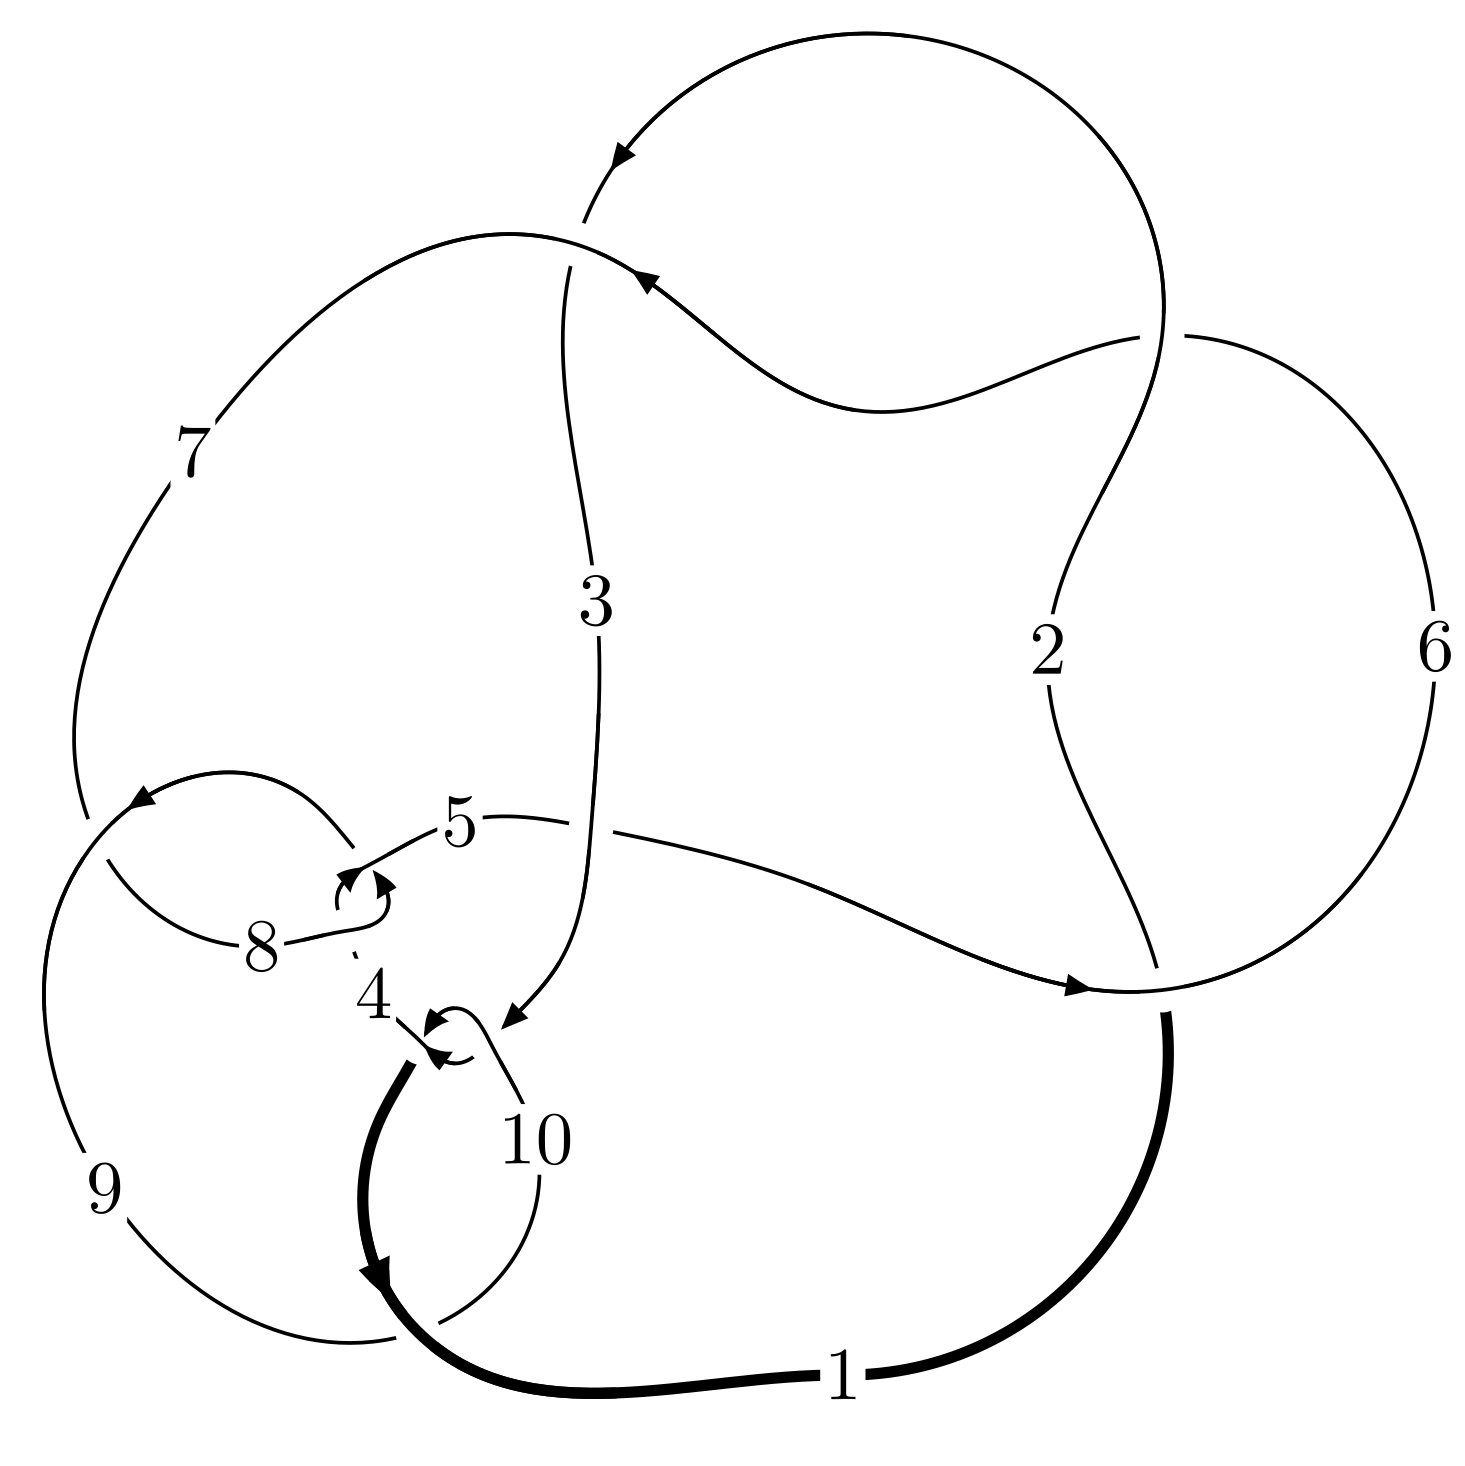
\includegraphics[width=112pt]{../../../GIT/diagram.site/Diagrams/png/150_10_66.png}\\
\ \ \ A knot diagram\footnotemark}&
\allowdisplaybreaks
\textbf{Linearized knot diagam} \\
\cline{2-2}
 &
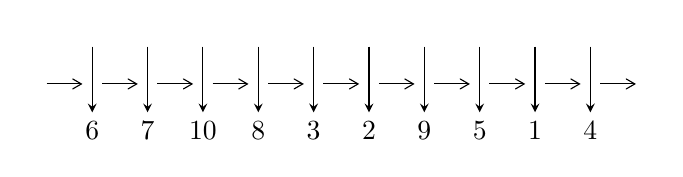
\begin{tikzpicture}[x=20pt, y=17pt]
	% nodes
	\node (C0) at (0, 0) {};
	\node (C1) at (1, 0) {};
	\node (C1U) at (1, +1) {};
	\node (C1D) at (1, -1) {6};

	\node (C2) at (2, 0) {};
	\node (C2U) at (2, +1) {};
	\node (C2D) at (2, -1) {7};

	\node (C3) at (3, 0) {};
	\node (C3U) at (3, +1) {};
	\node (C3D) at (3, -1) {10};

	\node (C4) at (4, 0) {};
	\node (C4U) at (4, +1) {};
	\node (C4D) at (4, -1) {8};

	\node (C5) at (5, 0) {};
	\node (C5U) at (5, +1) {};
	\node (C5D) at (5, -1) {3};

	\node (C6) at (6, 0) {};
	\node (C6U) at (6, +1) {};
	\node (C6D) at (6, -1) {2};

	\node (C7) at (7, 0) {};
	\node (C7U) at (7, +1) {};
	\node (C7D) at (7, -1) {9};

	\node (C8) at (8, 0) {};
	\node (C8U) at (8, +1) {};
	\node (C8D) at (8, -1) {5};

	\node (C9) at (9, 0) {};
	\node (C9U) at (9, +1) {};
	\node (C9D) at (9, -1) {1};

	\node (C10) at (10, 0) {};
	\node (C10U) at (10, +1) {};
	\node (C10D) at (10, -1) {4};
	\node (C11) at (11, 0) {};

	% arrows
	\draw[->,>={angle 60}]
	(C0) edge (C1) (C1) edge (C2) (C2) edge (C3) (C3) edge (C4) (C4) edge (C5) (C5) edge (C6) (C6) edge (C7) (C7) edge (C8) (C8) edge (C9) (C9) edge (C10) (C10) edge (C11) ;	\draw[->,>=stealth]
	(C1U) edge (C1D) (C2U) edge (C2D) (C3U) edge (C3D) (C4U) edge (C4D) (C5U) edge (C5D) (C6U) edge (C6D) (C7U) edge (C7D) (C8U) edge (C8D) (C9U) edge (C9D) (C10U) edge (C10D) ;
	\end{tikzpicture} \\
\hhline{~~} \\& 
\textbf{Solving Sequence} \\ \cline{2-2} 
 &
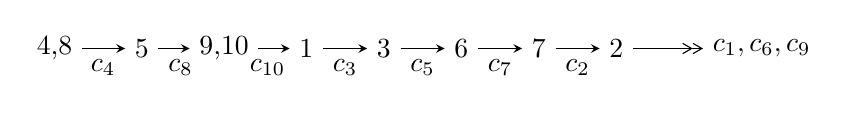
\begin{tikzpicture}[x=28pt, y=7pt]
	% node
	\node (A0) at (-1/8, 0) {4,8};
	\node (A1) at (1, 0) {5};
	\node (A2) at (33/16, 0) {9,10};
	\node (A3) at (25/8, 0) {1};
	\node (A4) at (33/8, 0) {3};
	\node (A5) at (41/8, 0) {6};
	\node (A6) at (49/8, 0) {7};
	\node (A7) at (57/8, 0) {2};
	\node (C1) at (1/2, -1) {$c_{4}$};
	\node (C2) at (3/2, -1) {$c_{8}$};
	\node (C3) at (21/8, -1) {$c_{10}$};
	\node (C4) at (29/8, -1) {$c_{3}$};
	\node (C5) at (37/8, -1) {$c_{5}$};
	\node (C6) at (45/8, -1) {$c_{7}$};
	\node (C7) at (53/8, -1) {$c_{2}$};
	\node (A8) at (9, 0) {$c_{1},c_{6},c_{9}$};

	% edge
	\draw[->,>=stealth]	
	(A0) edge (A1) (A1) edge (A2) (A2) edge (A3) (A3) edge (A4) (A4) edge (A5) (A5) edge (A6) (A6) edge (A7) ;
	\draw[->>,>={angle 60}]	
	(A7) edge (A8);
\end{tikzpicture} \\ 

\end{tabular} \\

\footnotetext{
The image of knot diagram is generated by the software ``\textbf{Draw programme}" developed by Andrew Bartholomew(\url{http://www.layer8.co.uk/maths/draw/index.htm\#Running-draw}), where we modified some parts for our purpose(\url{https://github.com/CATsTAILs/LinksPainter}).
}\phantom \\ \newline 
\centering \textbf{Ideals for irreducible components\footnotemark of $X_{\text{par}}$} 
 
\begin{align*}
I^u_{1}&=\langle 
b- u,\;u^{15}+u^{14}-2 u^{13}-3 u^{12}+4 u^{11}+6 u^{10}- u^9-6 u^8+2 u^7+5 u^6+3 u^5-3 u^4+2 u^3+2 u^2+2 a+3 u,\\
\phantom{I^u_{1}}&\phantom{= \langle  }u^{16}+u^{15}-3 u^{14}-4 u^{13}+6 u^{12}+9 u^{11}-5 u^{10}-12 u^9+3 u^8+11 u^7+u^6-8 u^5- u^4+5 u^3+3 u^2-2 u-1\rangle \\
I^u_{2}&=\langle 
11603 u^{23}+6022 u^{22}+\cdots+8177 b+4273,\;3426 u^{23}-2155 u^{22}+\cdots+8177 a-28435,\\
\phantom{I^u_{2}}&\phantom{= \langle  }u^{24}+u^{23}+\cdots+4 u+1\rangle \\
I^u_{3}&=\langle 
b-1,\;a^2-4 a+2,\;u+1\rangle \\
I^u_{4}&=\langle 
b+1,\;a+2,\;u-1\rangle \\
\\
\end{align*}
\raggedright * 4 irreducible components of $\dim_{\mathbb{C}}=0$, with total 43 representations.\\
\footnotetext{All coefficients of polynomials are rational numbers. But the coefficients are sometimes approximated in decimal forms when there is not enough margin.}
\newpage
\renewcommand{\arraystretch}{1}
\centering \section*{I. $I^u_{1}= \langle b- u,\;u^{15}+u^{14}+\cdots+2 a+3 u,\;u^{16}+u^{15}+\cdots-2 u-1 \rangle$}
\flushleft \textbf{(i) Arc colorings}\\
\begin{tabular}{m{7pt} m{180pt} m{7pt} m{180pt} }
\flushright $a_{4}=$&$\begin{pmatrix}1\\0\end{pmatrix}$ \\
\flushright $a_{8}=$&$\begin{pmatrix}0\\u\end{pmatrix}$ \\
\flushright $a_{5}=$&$\begin{pmatrix}1\\u^2\end{pmatrix}$ \\
\flushright $a_{9}=$&$\begin{pmatrix}- u\\- u^3+u\end{pmatrix}$ \\
\flushright $a_{10}=$&$\begin{pmatrix}-\frac{1}{2} u^{15}-\frac{1}{2} u^{14}+\cdots- u^2-\frac{3}{2} u\\u\end{pmatrix}$ \\
\flushright $a_{1}=$&$\begin{pmatrix}-\frac{1}{2} u^{15}-\frac{1}{2} u^{14}+\cdots- u^2-\frac{5}{2} u\\u\end{pmatrix}$ \\
\flushright $a_{3}=$&$\begin{pmatrix}\frac{1}{2} u^{14}+\frac{1}{2} u^{13}+\cdots+u+\frac{3}{2}\\- u^2\end{pmatrix}$ \\
\flushright $a_{6}=$&$\begin{pmatrix}-\frac{1}{2} u^{15}-\frac{3}{2} u^{14}+\cdots-\frac{9}{2} u-1\\\frac{1}{2} u^{14}+\frac{1}{2} u^{13}+\cdots+u+\frac{1}{2}\end{pmatrix}$ \\
\flushright $a_{7}=$&$\begin{pmatrix}u^3\\u^5- u^3+u\end{pmatrix}$ \\
\flushright $a_{2}=$&$\begin{pmatrix}u^{10}- u^8+2 u^6+u^4+u^2+1\\-\frac{1}{2} u^{14}-\frac{1}{2} u^{13}+\cdots- u-\frac{1}{2}\end{pmatrix}$\\&\end{tabular}
\flushleft \textbf{(ii) Obstruction class $= -1$}\\~\\
\flushleft \textbf{(iii) Cusp Shapes $= u^{15}+u^{14}-4 u^{13}-3 u^{12}+12 u^{11}+8 u^{10}-19 u^9-12 u^8+22 u^7+17 u^6-13 u^5-13 u^4+6 u^3+12 u^2- u-16$}\\~\\
\newpage\renewcommand{\arraystretch}{1}
\flushleft \textbf{(iv) u-Polynomials at the component}\newline \\
\begin{tabular}{m{50pt}|m{274pt}}
Crossings & \hspace{64pt}u-Polynomials at each crossing \\
\hline $$\begin{aligned}c_{1},c_{2},c_{6}\end{aligned}$$&$\begin{aligned}
&u^{16}+3 u^{15}+\cdots-2 u-2
\end{aligned}$\\
\hline $$\begin{aligned}c_{3},c_{4},c_{8}\\c_{10}\end{aligned}$$&$\begin{aligned}
&u^{16}+u^{15}+\cdots-2 u-1
\end{aligned}$\\
\hline $$\begin{aligned}c_{5}\end{aligned}$$&$\begin{aligned}
&u^{16}-9 u^{15}+\cdots-34 u+14
\end{aligned}$\\
\hline $$\begin{aligned}c_{7},c_{9}\end{aligned}$$&$\begin{aligned}
&u^{16}+7 u^{15}+\cdots+10 u+1
\end{aligned}$\\
\hline
\end{tabular}\\~\\
\newpage\renewcommand{\arraystretch}{1}
\flushleft \textbf{(v) Riley Polynomials at the component}\newline \\
\begin{tabular}{m{50pt}|m{274pt}}
Crossings & \hspace{64pt}Riley Polynomials at each crossing \\
\hline $$\begin{aligned}c_{1},c_{2},c_{6}\end{aligned}$$&$\begin{aligned}
&y^{16}-15 y^{15}+\cdots-20 y+4
\end{aligned}$\\
\hline $$\begin{aligned}c_{3},c_{4},c_{8}\\c_{10}\end{aligned}$$&$\begin{aligned}
&y^{16}-7 y^{15}+\cdots-10 y+1
\end{aligned}$\\
\hline $$\begin{aligned}c_{5}\end{aligned}$$&$\begin{aligned}
&y^{16}-3 y^{15}+\cdots-1156 y+196
\end{aligned}$\\
\hline $$\begin{aligned}c_{7},c_{9}\end{aligned}$$&$\begin{aligned}
&y^{16}+9 y^{15}+\cdots-38 y+1
\end{aligned}$\\
\hline
\end{tabular}\\~\\
\newpage\flushleft \textbf{(vi) Complex Volumes and Cusp Shapes}
$$\begin{array}{c|c|c}  
\text{Solutions to }I^u_{1}& \I (\text{vol} + \sqrt{-1}CS) & \text{Cusp shape}\\
 \hline 
\begin{aligned}
u &= -0.788317 + 0.682807 I \\
a &= -0.862130 - 0.839659 I \\
b &= -0.788317 + 0.682807 I\end{aligned}
 & -0.17586 + 4.85157 I & -10.18415 - 6.53900 I \\ \hline\begin{aligned}
u &= -0.788317 - 0.682807 I \\
a &= -0.862130 + 0.839659 I \\
b &= -0.788317 - 0.682807 I\end{aligned}
 & -0.17586 - 4.85157 I & -10.18415 + 6.53900 I \\ \hline\begin{aligned}
u &= \phantom{-}0.591599 + 0.705742 I \\
a &= \phantom{-}0.502397 - 0.588564 I \\
b &= \phantom{-}0.591599 + 0.705742 I\end{aligned}
 & \phantom{-}3.06515 - 1.13134 I & -4.88295 + 2.50814 I \\ \hline\begin{aligned}
u &= \phantom{-}0.591599 - 0.705742 I \\
a &= \phantom{-}0.502397 + 0.588564 I \\
b &= \phantom{-}0.591599 - 0.705742 I\end{aligned}
 & \phantom{-}3.06515 + 1.13134 I & -4.88295 - 2.50814 I \\ \hline\begin{aligned}
u &= -0.403938 + 0.782402 I \\
a &= -0.331306 - 0.329211 I \\
b &= -0.403938 + 0.782402 I\end{aligned}
 & -1.21964 - 2.39915 I & -9.20728 + 0.67092 I \\ \hline\begin{aligned}
u &= -0.403938 - 0.782402 I \\
a &= -0.331306 + 0.329211 I \\
b &= -0.403938 - 0.782402 I\end{aligned}
 & -1.21964 + 2.39915 I & -9.20728 - 0.67092 I \\ \hline\begin{aligned}
u &= \phantom{-}1.043770 + 0.418403 I \\
a &= \phantom{-}1.76067 - 2.04191 I \\
b &= \phantom{-}1.043770 + 0.418403 I\end{aligned}
 & -8.80698 - 2.79176 I & -16.7106 + 5.2072 I \\ \hline\begin{aligned}
u &= \phantom{-}1.043770 - 0.418403 I \\
a &= \phantom{-}1.76067 + 2.04191 I \\
b &= \phantom{-}1.043770 - 0.418403 I\end{aligned}
 & -8.80698 + 2.79176 I & -16.7106 - 5.2072 I \\ \hline\begin{aligned}
u &= -1.034800 + 0.560504 I \\
a &= -1.60194 - 1.34258 I \\
b &= -1.034800 + 0.560504 I\end{aligned}
 & -1.63698 + 4.78532 I & -12.50670 - 3.64348 I \\ \hline\begin{aligned}
u &= -1.034800 - 0.560504 I \\
a &= -1.60194 + 1.34258 I \\
b &= -1.034800 - 0.560504 I\end{aligned}
 & -1.63698 - 4.78532 I & -12.50670 + 3.64348 I\\
 \hline 
 \end{array}$$\newpage$$\begin{array}{c|c|c}  
\text{Solutions to }I^u_{1}& \I (\text{vol} + \sqrt{-1}CS) & \text{Cusp shape}\\
 \hline 
\begin{aligned}
u &= \phantom{-}1.123030 + 0.603482 I \\
a &= \phantom{-}1.88319 - 1.11133 I \\
b &= \phantom{-}1.123030 + 0.603482 I\end{aligned}
 & -0.34351 - 9.16484 I & -10.75715 + 8.12303 I \\ \hline\begin{aligned}
u &= \phantom{-}1.123030 - 0.603482 I \\
a &= \phantom{-}1.88319 + 1.11133 I \\
b &= \phantom{-}1.123030 - 0.603482 I\end{aligned}
 & -0.34351 + 9.16484 I & -10.75715 - 8.12303 I \\ \hline\begin{aligned}
u &= \phantom{-}0.703289\phantom{ +0.000000I} \\
a &= -2.07989\phantom{ +0.000000I} \\
b &= \phantom{-}0.703289\phantom{ +0.000000I}\end{aligned}
 & -6.93855\phantom{ +0.000000I} & -11.2730\phantom{ +0.000000I} \\ \hline\begin{aligned}
u &= -1.184280 + 0.595800 I \\
a &= -2.08419 - 1.05231 I \\
b &= -1.184280 + 0.595800 I\end{aligned}
 & -5.9872 + 13.0293 I & -14.9902 - 8.3428 I \\ \hline\begin{aligned}
u &= -1.184280 - 0.595800 I \\
a &= -2.08419 + 1.05231 I \\
b &= -1.184280 - 0.595800 I\end{aligned}
 & -5.9872 - 13.0293 I & -14.9902 + 8.3428 I \\ \hline\begin{aligned}
u &= -0.397419\phantom{ +0.000000I} \\
a &= \phantom{-}0.546503\phantom{ +0.000000I} \\
b &= -0.397419\phantom{ +0.000000I}\end{aligned}
 & -0.684897\phantom{ +0.000000I} & -14.2490\phantom{ +0.000000I}\\
 \hline 
 \end{array}$$\newpage\newpage\renewcommand{\arraystretch}{1}
\centering \section*{II. $I^u_{2}= \langle 11603 u^{23}+6022 u^{22}+\cdots+8177 b+4273,\;3426 u^{23}-2155 u^{22}+\cdots+8177 a-28435,\;u^{24}+u^{23}+\cdots+4 u+1 \rangle$}
\flushleft \textbf{(i) Arc colorings}\\
\begin{tabular}{m{7pt} m{180pt} m{7pt} m{180pt} }
\flushright $a_{4}=$&$\begin{pmatrix}1\\0\end{pmatrix}$ \\
\flushright $a_{8}=$&$\begin{pmatrix}0\\u\end{pmatrix}$ \\
\flushright $a_{5}=$&$\begin{pmatrix}1\\u^2\end{pmatrix}$ \\
\flushright $a_{9}=$&$\begin{pmatrix}- u\\- u^3+u\end{pmatrix}$ \\
\flushright $a_{10}=$&$\begin{pmatrix}-0.418980 u^{23}+0.263544 u^{22}+\cdots+0.0328972 u+3.47744\\-1.41898 u^{23}-0.736456 u^{22}+\cdots-5.96710 u-0.522563\end{pmatrix}$ \\
\flushright $a_{1}=$&$\begin{pmatrix}u^{23}+u^{22}+\cdots+6 u+4\\-1.41898 u^{23}-0.736456 u^{22}+\cdots-5.96710 u-0.522563\end{pmatrix}$ \\
\flushright $a_{3}=$&$\begin{pmatrix}1.20509 u^{23}-0.359300 u^{22}+\cdots+1.96025 u-2.45787\\0.682524 u^{23}+0.537116 u^{22}+\cdots+5.15336 u+0.418980\end{pmatrix}$ \\
\flushright $a_{6}=$&$\begin{pmatrix}-0.203987 u^{23}+1.29118 u^{22}+\cdots+4.42057 u+5.51266\\-0.997187 u^{23}-0.285190 u^{22}+\cdots-4.02678 u+0.362236\end{pmatrix}$ \\
\flushright $a_{7}=$&$\begin{pmatrix}u^3\\u^5- u^3+u\end{pmatrix}$ \\
\flushright $a_{2}=$&$\begin{pmatrix}1.12511 u^{23}-0.0760670 u^{22}+\cdots+0.287025 u-3.10578\\0.00195671 u^{23}+0.323346 u^{22}+\cdots-0.322979 u-0.791488\end{pmatrix}$\\&\end{tabular}
\flushleft \textbf{(ii) Obstruction class $= -1$}\\~\\
\flushleft \textbf{(iii) Cusp Shapes $= \frac{19748}{8177} u^{23}+\frac{17088}{8177} u^{22}+\cdots+\frac{29544}{8177} u-\frac{105438}{8177}$}\\~\\
\newpage\renewcommand{\arraystretch}{1}
\flushleft \textbf{(iv) u-Polynomials at the component}\newline \\
\begin{tabular}{m{50pt}|m{274pt}}
Crossings & \hspace{64pt}u-Polynomials at each crossing \\
\hline $$\begin{aligned}c_{1},c_{2},c_{6}\end{aligned}$$&$\begin{aligned}
&(u^{12}- u^{11}-5 u^{10}+4 u^9+9 u^8-4 u^7-6 u^6-2 u^5+3 u^3+u^2+1)^2
\end{aligned}$\\
\hline $$\begin{aligned}c_{3},c_{4},c_{8}\\c_{10}\end{aligned}$$&$\begin{aligned}
&u^{24}+u^{23}+\cdots+4 u+1
\end{aligned}$\\
\hline $$\begin{aligned}c_{5}\end{aligned}$$&$\begin{aligned}
&(u^{12}+3 u^{11}+\cdots+4 u+1)^{2}
\end{aligned}$\\
\hline $$\begin{aligned}c_{7},c_{9}\end{aligned}$$&$\begin{aligned}
&u^{24}+13 u^{23}+\cdots+4 u+1
\end{aligned}$\\
\hline
\end{tabular}\\~\\
\newpage\renewcommand{\arraystretch}{1}
\flushleft \textbf{(v) Riley Polynomials at the component}\newline \\
\begin{tabular}{m{50pt}|m{274pt}}
Crossings & \hspace{64pt}Riley Polynomials at each crossing \\
\hline $$\begin{aligned}c_{1},c_{2},c_{6}\end{aligned}$$&$\begin{aligned}
&(y^{12}-11 y^{11}+\cdots+2 y+1)^{2}
\end{aligned}$\\
\hline $$\begin{aligned}c_{3},c_{4},c_{8}\\c_{10}\end{aligned}$$&$\begin{aligned}
&y^{24}-13 y^{23}+\cdots-4 y+1
\end{aligned}$\\
\hline $$\begin{aligned}c_{5}\end{aligned}$$&$\begin{aligned}
&(y^{12}+y^{11}+\cdots-2 y+1)^{2}
\end{aligned}$\\
\hline $$\begin{aligned}c_{7},c_{9}\end{aligned}$$&$\begin{aligned}
&y^{24}-5 y^{23}+\cdots+48 y+1
\end{aligned}$\\
\hline
\end{tabular}\\~\\
\newpage\flushleft \textbf{(vi) Complex Volumes and Cusp Shapes}
$$\begin{array}{c|c|c}  
\text{Solutions to }I^u_{2}& \I (\text{vol} + \sqrt{-1}CS) & \text{Cusp shape}\\
 \hline 
\begin{aligned}
u &= \phantom{-}0.961597 + 0.331697 I \\
a &= -2.11926 + 0.49208 I \\
b &= -1.189900 + 0.171507 I\end{aligned}
 & -3.28987 - 1.20211 I & -12.00000 + 5.63740 I \\ \hline\begin{aligned}
u &= \phantom{-}0.961597 - 0.331697 I \\
a &= -2.11926 - 0.49208 I \\
b &= -1.189900 - 0.171507 I\end{aligned}
 & -3.28987 + 1.20211 I & -12.00000 - 5.63740 I \\ \hline\begin{aligned}
u &= -0.778724 + 0.569322 I \\
a &= \phantom{-}0.272376 - 0.021441 I \\
b &= -0.564477 - 0.633261 I\end{aligned}
 & -0.174773 + 0.093609 I & -10.00912 + 0.76204 I \\ \hline\begin{aligned}
u &= -0.778724 - 0.569322 I \\
a &= \phantom{-}0.272376 + 0.021441 I \\
b &= -0.564477 + 0.633261 I\end{aligned}
 & -0.174773 - 0.093609 I & -10.00912 - 0.76204 I \\ \hline\begin{aligned}
u &= -0.285725 + 0.889847 I \\
a &= -0.777424 + 0.420961 I \\
b &= -1.104540 - 0.597792 I\end{aligned}
 & -3.28987 - 7.58818 I & -12.00000 + 5.13539 I \\ \hline\begin{aligned}
u &= -0.285725 - 0.889847 I \\
a &= -0.777424 - 0.420961 I \\
b &= -1.104540 + 0.597792 I\end{aligned}
 & -3.28987 + 7.58818 I & -12.00000 - 5.13539 I \\ \hline\begin{aligned}
u &= \phantom{-}0.384175 + 0.809134 I \\
a &= \phantom{-}0.520131 + 0.408228 I \\
b &= \phantom{-}0.998981 - 0.600305 I\end{aligned}
 & \phantom{-}1.84911 + 3.88480 I & -7.19439 - 4.17140 I \\ \hline\begin{aligned}
u &= \phantom{-}0.384175 - 0.809134 I \\
a &= \phantom{-}0.520131 - 0.408228 I \\
b &= \phantom{-}0.998981 + 0.600305 I\end{aligned}
 & \phantom{-}1.84911 - 3.88480 I & -7.19439 + 4.17140 I \\ \hline\begin{aligned}
u &= -0.564477 + 0.633261 I \\
a &= \phantom{-}0.005650 + 0.310630 I \\
b &= -0.778724 - 0.569322 I\end{aligned}
 & -0.174773 - 0.093609 I & -10.00912 - 0.76204 I \\ \hline\begin{aligned}
u &= -0.564477 - 0.633261 I \\
a &= \phantom{-}0.005650 - 0.310630 I \\
b &= -0.778724 + 0.569322 I\end{aligned}
 & -0.174773 + 0.093609 I & -10.00912 + 0.76204 I\\
 \hline 
 \end{array}$$\newpage$$\begin{array}{c|c|c}  
\text{Solutions to }I^u_{2}& \I (\text{vol} + \sqrt{-1}CS) & \text{Cusp shape}\\
 \hline 
\begin{aligned}
u &= -1.057630 + 0.470734 I \\
a &= \phantom{-}2.07384 + 0.60989 I \\
b &= \phantom{-}1.284660 + 0.258642 I\end{aligned}
 & -8.42885 + 3.88480 I & -16.8056 - 4.1714 I \\ \hline\begin{aligned}
u &= -1.057630 - 0.470734 I \\
a &= \phantom{-}2.07384 - 0.60989 I \\
b &= \phantom{-}1.284660 - 0.258642 I\end{aligned}
 & -8.42885 - 3.88480 I & -16.8056 + 4.1714 I \\ \hline\begin{aligned}
u &= \phantom{-}0.998981 + 0.600305 I \\
a &= -0.351273 - 0.367190 I \\
b &= \phantom{-}0.384175 - 0.809134 I\end{aligned}
 & \phantom{-}1.84911 - 3.88480 I & -7.19439 + 4.17140 I \\ \hline\begin{aligned}
u &= \phantom{-}0.998981 - 0.600305 I \\
a &= -0.351273 + 0.367190 I \\
b &= \phantom{-}0.384175 + 0.809134 I\end{aligned}
 & \phantom{-}1.84911 + 3.88480 I & -7.19439 - 4.17140 I \\ \hline\begin{aligned}
u &= \phantom{-}1.165410 + 0.089633 I \\
a &= -1.166860 - 0.270592 I \\
b &= -0.313835 - 0.336199 I\end{aligned}
 & -6.40496 + 0.09361 I & -13.99088 + 0.76204 I \\ \hline\begin{aligned}
u &= \phantom{-}1.165410 - 0.089633 I \\
a &= -1.166860 + 0.270592 I \\
b &= -0.313835 + 0.336199 I\end{aligned}
 & -6.40496 - 0.09361 I & -13.99088 - 0.76204 I \\ \hline\begin{aligned}
u &= -1.189900 + 0.171507 I \\
a &= \phantom{-}1.78490 + 0.45036 I \\
b &= \phantom{-}0.961597 + 0.331697 I\end{aligned}
 & -3.28987 - 1.20211 I & -12.00000 + 5.63740 I \\ \hline\begin{aligned}
u &= -1.189900 - 0.171507 I \\
a &= \phantom{-}1.78490 - 0.45036 I \\
b &= \phantom{-}0.961597 - 0.331697 I\end{aligned}
 & -3.28987 + 1.20211 I & -12.00000 - 5.63740 I \\ \hline\begin{aligned}
u &= -1.104540 + 0.597792 I \\
a &= \phantom{-}0.414520 - 0.510865 I \\
b &= -0.285725 - 0.889847 I\end{aligned}
 & -3.28987 + 7.58818 I & -12.00000 - 5.13539 I \\ \hline\begin{aligned}
u &= -1.104540 - 0.597792 I \\
a &= \phantom{-}0.414520 + 0.510865 I \\
b &= -0.285725 + 0.889847 I\end{aligned}
 & -3.28987 - 7.58818 I & -12.00000 + 5.13539 I\\
 \hline 
 \end{array}$$\newpage$$\begin{array}{c|c|c}  
\text{Solutions to }I^u_{2}& \I (\text{vol} + \sqrt{-1}CS) & \text{Cusp shape}\\
 \hline 
\begin{aligned}
u &= \phantom{-}1.284660 + 0.258642 I \\
a &= -1.80572 + 0.62135 I \\
b &= -1.057630 + 0.470734 I\end{aligned}
 & -8.42885 + 3.88480 I & -16.8056 - 4.1714 I \\ \hline\begin{aligned}
u &= \phantom{-}1.284660 - 0.258642 I \\
a &= -1.80572 - 0.62135 I \\
b &= -1.057630 - 0.470734 I\end{aligned}
 & -8.42885 - 3.88480 I & -16.8056 + 4.1714 I \\ \hline\begin{aligned}
u &= -0.313835 + 0.336199 I \\
a &= \phantom{-}2.64911 + 1.49979 I \\
b &= \phantom{-}1.165410 - 0.089633 I\end{aligned}
 & -6.40496 - 0.09361 I & -13.99088 - 0.76204 I \\ \hline\begin{aligned}
u &= -0.313835 - 0.336199 I \\
a &= \phantom{-}2.64911 - 1.49979 I \\
b &= \phantom{-}1.165410 + 0.089633 I\end{aligned}
 & -6.40496 + 0.09361 I & -13.99088 + 0.76204 I\\
 \hline 
 \end{array}$$\newpage\newpage\renewcommand{\arraystretch}{1}
\centering \section*{III. $I^u_{3}= \langle b-1,\;a^2-4 a+2,\;u+1 \rangle$}
\flushleft \textbf{(i) Arc colorings}\\
\begin{tabular}{m{7pt} m{180pt} m{7pt} m{180pt} }
\flushright $a_{4}=$&$\begin{pmatrix}1\\0\end{pmatrix}$ \\
\flushright $a_{8}=$&$\begin{pmatrix}0\\-1\end{pmatrix}$ \\
\flushright $a_{5}=$&$\begin{pmatrix}1\\1\end{pmatrix}$ \\
\flushright $a_{9}=$&$\begin{pmatrix}1\\0\end{pmatrix}$ \\
\flushright $a_{10}=$&$\begin{pmatrix}a\\1\end{pmatrix}$ \\
\flushright $a_{1}=$&$\begin{pmatrix}a-1\\1\end{pmatrix}$ \\
\flushright $a_{3}=$&$\begin{pmatrix}- a+1\\-1\end{pmatrix}$ \\
\flushright $a_{6}=$&$\begin{pmatrix}- a+1\\- a+3\end{pmatrix}$ \\
\flushright $a_{7}=$&$\begin{pmatrix}-1\\-1\end{pmatrix}$ \\
\flushright $a_{2}=$&$\begin{pmatrix}-1\\a-3\end{pmatrix}$\\&\end{tabular}
\flushleft \textbf{(ii) Obstruction class $= 1$}\\~\\
\flushleft \textbf{(iii) Cusp Shapes $= -20$}\\~\\
\newpage\renewcommand{\arraystretch}{1}
\flushleft \textbf{(iv) u-Polynomials at the component}\newline \\
\begin{tabular}{m{50pt}|m{274pt}}
Crossings & \hspace{64pt}u-Polynomials at each crossing \\
\hline $$\begin{aligned}c_{1},c_{2},c_{5}\\c_{6}\end{aligned}$$&$\begin{aligned}
&u^2-2
\end{aligned}$\\
\hline $$\begin{aligned}c_{3},c_{7},c_{8}\\c_{9}\end{aligned}$$&$\begin{aligned}
&(u-1)^2
\end{aligned}$\\
\hline $$\begin{aligned}c_{4},c_{10}\end{aligned}$$&$\begin{aligned}
&(u+1)^2
\end{aligned}$\\
\hline
\end{tabular}\\~\\
\newpage\renewcommand{\arraystretch}{1}
\flushleft \textbf{(v) Riley Polynomials at the component}\newline \\
\begin{tabular}{m{50pt}|m{274pt}}
Crossings & \hspace{64pt}Riley Polynomials at each crossing \\
\hline $$\begin{aligned}c_{1},c_{2},c_{5}\\c_{6}\end{aligned}$$&$\begin{aligned}
&(y-2)^2
\end{aligned}$\\
\hline $$\begin{aligned}c_{3},c_{4},c_{7}\\c_{8},c_{9},c_{10}\end{aligned}$$&$\begin{aligned}
&(y-1)^2
\end{aligned}$\\
\hline
\end{tabular}\\~\\
\newpage\flushleft \textbf{(vi) Complex Volumes and Cusp Shapes}
$$\begin{array}{c|c|c}  
\text{Solutions to }I^u_{3}& \I (\text{vol} + \sqrt{-1}CS) & \text{Cusp shape}\\
 \hline 
\begin{aligned}
u &= -1.00000\phantom{ +0.000000I} \\
a &= \phantom{-}0.585786\phantom{ +0.000000I} \\
b &= \phantom{-}1.00000\phantom{ +0.000000I}\end{aligned}
 & -8.22467\phantom{ +0.000000I} & -20.0000\phantom{ +0.000000I} \\ \hline\begin{aligned}
u &= -1.00000\phantom{ +0.000000I} \\
a &= \phantom{-}3.41421\phantom{ +0.000000I} \\
b &= \phantom{-}1.00000\phantom{ +0.000000I}\end{aligned}
 & -8.22467\phantom{ +0.000000I} & -20.0000\phantom{ +0.000000I}\\
 \hline 
 \end{array}$$\newpage\newpage\renewcommand{\arraystretch}{1}
\centering \section*{IV. $I^u_{4}= \langle b+1,\;a+2,\;u-1 \rangle$}
\flushleft \textbf{(i) Arc colorings}\\
\begin{tabular}{m{7pt} m{180pt} m{7pt} m{180pt} }
\flushright $a_{4}=$&$\begin{pmatrix}1\\0\end{pmatrix}$ \\
\flushright $a_{8}=$&$\begin{pmatrix}0\\1\end{pmatrix}$ \\
\flushright $a_{5}=$&$\begin{pmatrix}1\\1\end{pmatrix}$ \\
\flushright $a_{9}=$&$\begin{pmatrix}-1\\0\end{pmatrix}$ \\
\flushright $a_{10}=$&$\begin{pmatrix}-2\\-1\end{pmatrix}$ \\
\flushright $a_{1}=$&$\begin{pmatrix}-1\\-1\end{pmatrix}$ \\
\flushright $a_{3}=$&$\begin{pmatrix}-1\\-1\end{pmatrix}$ \\
\flushright $a_{6}=$&$\begin{pmatrix}1\\1\end{pmatrix}$ \\
\flushright $a_{7}=$&$\begin{pmatrix}1\\1\end{pmatrix}$ \\
\flushright $a_{2}=$&$\begin{pmatrix}-1\\-1\end{pmatrix}$\\&\end{tabular}
\flushleft \textbf{(ii) Obstruction class $= 1$}\\~\\
\flushleft \textbf{(iii) Cusp Shapes $= -12$}\\~\\
\newpage\renewcommand{\arraystretch}{1}
\flushleft \textbf{(iv) u-Polynomials at the component}\newline \\
\begin{tabular}{m{50pt}|m{274pt}}
Crossings & \hspace{64pt}u-Polynomials at each crossing \\
\hline $$\begin{aligned}c_{1},c_{2},c_{5}\\c_{6}\end{aligned}$$&$\begin{aligned}
&u
\end{aligned}$\\
\hline $$\begin{aligned}c_{3},c_{8}\end{aligned}$$&$\begin{aligned}
&u+1
\end{aligned}$\\
\hline $$\begin{aligned}c_{4},c_{7},c_{9}\\c_{10}\end{aligned}$$&$\begin{aligned}
&u-1
\end{aligned}$\\
\hline
\end{tabular}\\~\\
\newpage\renewcommand{\arraystretch}{1}
\flushleft \textbf{(v) Riley Polynomials at the component}\newline \\
\begin{tabular}{m{50pt}|m{274pt}}
Crossings & \hspace{64pt}Riley Polynomials at each crossing \\
\hline $$\begin{aligned}c_{1},c_{2},c_{5}\\c_{6}\end{aligned}$$&$\begin{aligned}
&y
\end{aligned}$\\
\hline $$\begin{aligned}c_{3},c_{4},c_{7}\\c_{8},c_{9},c_{10}\end{aligned}$$&$\begin{aligned}
&y-1
\end{aligned}$\\
\hline
\end{tabular}\\~\\
\newpage\flushleft \textbf{(vi) Complex Volumes and Cusp Shapes}
$$\begin{array}{c|c|c}  
\text{Solutions to }I^u_{4}& \I (\text{vol} + \sqrt{-1}CS) & \text{Cusp shape}\\
 \hline 
\begin{aligned}
u &= \phantom{-}1.00000\phantom{ +0.000000I} \\
a &= -2.00000\phantom{ +0.000000I} \\
b &= -1.00000\phantom{ +0.000000I}\end{aligned}
 & -3.28987\phantom{ +0.000000I} & -12.0000\phantom{ +0.000000I}\\
 \hline 
 \end{array}$$\newpage
\newpage\renewcommand{\arraystretch}{1}
\centering \section*{ V. u-Polynomials}
\begin{tabular}{m{50pt}|m{274pt}}
Crossings & \hspace{64pt}u-Polynomials at each crossing \\
\hline $$\begin{aligned}c_{1},c_{2},c_{6}\end{aligned}$$&$\begin{aligned}
&u(u^2-2)(u^{12}- u^{11}+\cdots+u^2+1)^{2}\\
&\cdot(u^{16}+3 u^{15}+\cdots-2 u-2)
\end{aligned}$\\
\hline $$\begin{aligned}c_{3},c_{8}\end{aligned}$$&$\begin{aligned}
&((u-1)^2)(u+1)(u^{16}+u^{15}+\cdots-2 u-1)(u^{24}+u^{23}+\cdots+4 u+1)
\end{aligned}$\\
\hline $$\begin{aligned}c_{4},c_{10}\end{aligned}$$&$\begin{aligned}
&(u-1)(u+1)^2(u^{16}+u^{15}+\cdots-2 u-1)(u^{24}+u^{23}+\cdots+4 u+1)
\end{aligned}$\\
\hline $$\begin{aligned}c_{5}\end{aligned}$$&$\begin{aligned}
&u(u^2-2)(u^{12}+3 u^{11}+\cdots+4 u+1)^{2}(u^{16}-9 u^{15}+\cdots-34 u+14)
\end{aligned}$\\
\hline $$\begin{aligned}c_{7},c_{9}\end{aligned}$$&$\begin{aligned}
&((u-1)^3)(u^{16}+7 u^{15}+\cdots+10 u+1)(u^{24}+13 u^{23}+\cdots+4 u+1)
\end{aligned}$\\
\hline
\end{tabular}\newpage\renewcommand{\arraystretch}{1}
\centering \section*{ VI. Riley Polynomials}
\begin{tabular}{m{50pt}|m{274pt}}
Crossings & \hspace{64pt}Riley Polynomials at each crossing \\
\hline $$\begin{aligned}c_{1},c_{2},c_{6}\end{aligned}$$&$\begin{aligned}
&y(y-2)^2(y^{12}-11 y^{11}+\cdots+2 y+1)^{2}(y^{16}-15 y^{15}+\cdots-20 y+4)
\end{aligned}$\\
\hline $$\begin{aligned}c_{3},c_{4},c_{8}\\c_{10}\end{aligned}$$&$\begin{aligned}
&((y-1)^3)(y^{16}-7 y^{15}+\cdots-10 y+1)(y^{24}-13 y^{23}+\cdots-4 y+1)
\end{aligned}$\\
\hline $$\begin{aligned}c_{5}\end{aligned}$$&$\begin{aligned}
&y(y-2)^2(y^{12}+y^{11}+\cdots-2 y+1)^{2}\\
&\cdot(y^{16}-3 y^{15}+\cdots-1156 y+196)
\end{aligned}$\\
\hline $$\begin{aligned}c_{7},c_{9}\end{aligned}$$&$\begin{aligned}
&((y-1)^3)(y^{16}+9 y^{15}+\cdots-38 y+1)(y^{24}-5 y^{23}+\cdots+48 y+1)
\end{aligned}$\\
\hline
\end{tabular}
\vskip 2pc
\end{document}